\section{Clustering}

\subsection{K-means Clustering (14 points)}

\begin{enumerate}

\item \textbf{(6 Points)}
Given $n$ observations $X_1^n = \{X_1, \dots, X_n\}$, $X_i \in \Xcal$, the K-means objective
is to find $k$
($<n$) centres $\mu_1^k = \{\mu_1, \dots, \mu_k\}$, and a rule $f:\Xcal \rightarrow
\{1,\dots, K\}$ so as to minimize the objective

\begin{equation}
J(\mu_1^K, f; X_1^n) = \sum_{i=1}^n \sum_{k=1}^K \indfone(f(X_i) = k) \|X_i - \mu_k\|^2
\label{eqn:kmeans}
\end{equation}

Let $\Jcal_K(X_1^n) = \min_{\mu_1^k, f} J(\mu_1^K, f; X_1^n)$. Prove that
$\Jcal_{K}(X_1^n)$ is a non-increasing function of $K$.

\begin{soln}
    Prove via induction. 
    Suppose $K = 1$. 
    Now add one additional center so $K = 2$.
    If $\mu_2 = \mu_1$ then every $X_i$ is equal and $\Jcal_1(X_1^n) = \Jcal_2(X_1^n)$.
    Otherwise, if $\mu_2 \neq \mu_1$ then at least one $X_i \in \Xcal$ is closer to $\mu_2$ than $\mu_1$, thus $\Jcal_1(X_1^n) > \Jcal_2(X_1^n)$.
    So $\Jcal_{K}(X_1^n)$ is a non-increasing function of $K$ when $K = 1$.
    Now assume $\Jcal_{K}(X_1^n)$ is a non-increasing function of $K$ for $K = 1, 2, \dots, k$.
    Now consider $K = k + 1$.
    If $\exists i$ s.t. $\mu_i = \mu_{k+1}$, $i = 1, \dots, k$, then every $X_i$ is equal to some $\mu_i$ and $\Jcal_k(X_1^n) = \Jcal_{k+1}(X_1^n)$.
    Otherwise, if $\mu_{k+1} \neq \mu_i \forall i = 1, \dots, k$ then at least one $X_i \in \Xcal$ is closer to $\mu_{k+1}$ than any other $\mu_i$, thus $\Jcal_k(X_1^n) > \Jcal_{k+1}(X_1^n)$.
    So $\Jcal_{K}(X_1^n)$ is a non-increasing function of $K$ for any $K$.
\end{soln}

\item \textbf{(8 Points)}
Consider the K-means (Lloyd's) clustering algorithm we studied in class. We
terminate the algorithm when there are no changes to the objective.
Show that the algorithm terminates in a finite number of steps.

\begin{soln}
    First, prove the objective function in Lloyd's algorithm is strictly decreasing.
    Indeed, much like the EM algorithm, at each iteration Lloyd's algorithm finds the expected group of each observation and then maximizes the likelihood by moving the center to the optimal point among the points in its custer.
    This maximization step guarantees the objective function will decrease in the next iteration of the algorithm will terminate.
    Next, prove the Lloyd's algorithm will either terminate after finitely many steps or loop indefinitely.
    There are a finite number of data points, therefore, there are a finite number of ways observations can be partitioned.
    It follows that Lloyd's algorithm much terminate after finitely many steps or loop indefinitely.
    But since the objective function is strictly decreasing, the algorithm cannot loop indefinitely.
    Indeed, say at step $t$ the value of the objective function is $k_t$.
    Then, $k_{t+q} < k_{t}$ for $q = 1, 2, \dots$.
    But if the algorithm loops after $q$ iterations, then $k_t = k_{t + q}$ which is a contradiction.
    So Lloyd's algorithm cannot loop indefinitely, so it must terminate after finitely many iterations.
\end{soln}

\end{enumerate}



\subsection{Experiment (20 Points)}

In this question, we will evaluate
K-means clustering and GMM on a simple 2 dimensional problem.
First, create a two-dimensional synthetic dataset of 300 points by sampling 100 points each from the
three Gaussian distributions shown below:
\[
P_a = \Ncal\left(
\begin{bmatrix}
-1 \\ -1
\end{bmatrix},
\;
\sigma\begin{bmatrix}
2, &0.5 \\ 0.5, &1
\end{bmatrix}
\right),
\quad
P_b = \Ncal\left(
\begin{bmatrix}
1 \\ -1
\end{bmatrix},
\;
 \sigma\begin{bmatrix}
1, &-0.5 \\ -0.5, &2
\end{bmatrix}
\right),
\quad
P_c = \Ncal\left(
\begin{bmatrix}
0 \\ 1
\end{bmatrix},
\;
 \sigma\begin{bmatrix}
1 &0 \\ 0, &2
\end{bmatrix}
\right)
\]
Here, $\sigma$ is a parameter we will change to produce different datasets.

\begin{itemize}
\item First implement K-means clustering and the expectation maximization algorithm for GMMs.
Execute both methods on five synthetic datasets,
generated as shown above with $\sigma \in \{0.5, 1, 2, 4, 8\}$. Finally, evaluate both methods on \emph{(i)} the clustering objective~\eqref{eqn:kmeans} and \emph{(ii)}  the clustering accuracy. For each of the two criteria, plot the value achieved by each method against $\sigma$.

\item Both algorithms are only guaranteed to find only a local optimum so we recommend trying multiple
restarts and picking the one with the lowest objective value (This is~\eqref{eqn:kmeans} for K-means and the negative log likelihood for GMMs).
You may also experiment with a smart initialization
strategy (such as kmeans++).

\item
To plot the clustering accuracy,  you may treat the `label' of points generated from distribution
$P_u$ as $u$, where $u\in \{a, b, c\}$.
Assume that the cluster id $i$ returned by a method is $i\in \{1, 2, 3\}$.
Since clustering is an unsupervised learning problem, you should obtain the best possible mapping
from $\{1, 2, 3\}$ to $\{a, b, c\}$ to compute the clustering objective.
One way to do this is to compare the clustering centers returned by the method (centroids for
K-means, means for GMMs) and map them to the distribution with the closest mean.

\end{itemize}

Points break down: 7 points each for implementation of each method, 6 points for reporting of
evaluation metrics.

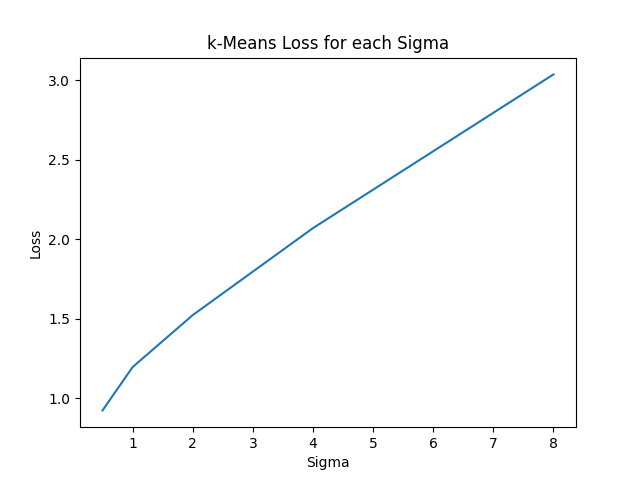
\includegraphics[width=3.15in]{../figs/kmeans_loss.png} \hspace{0.1in}
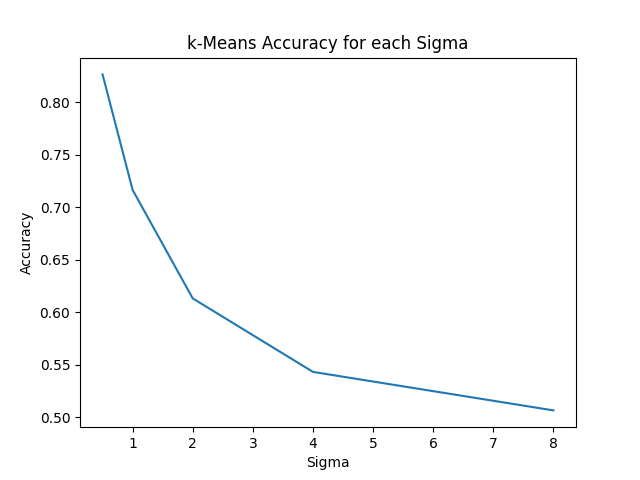
\includegraphics[width=3.15in]{../figs/kmeans_accuracy.png} \\

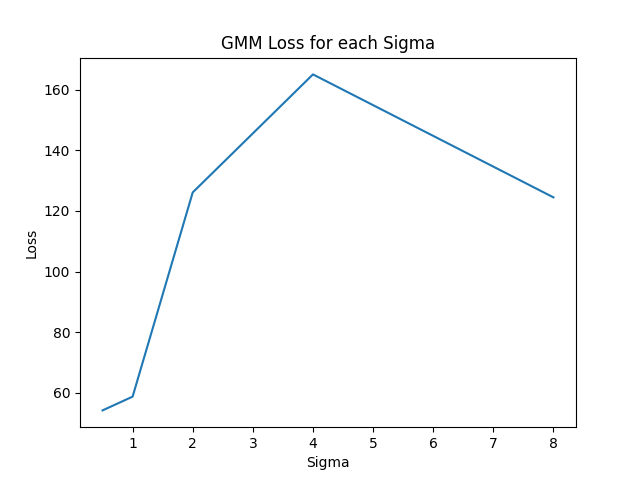
\includegraphics[width=3.15in]{../figs/gmm_loss.png} \hspace{0.1in}
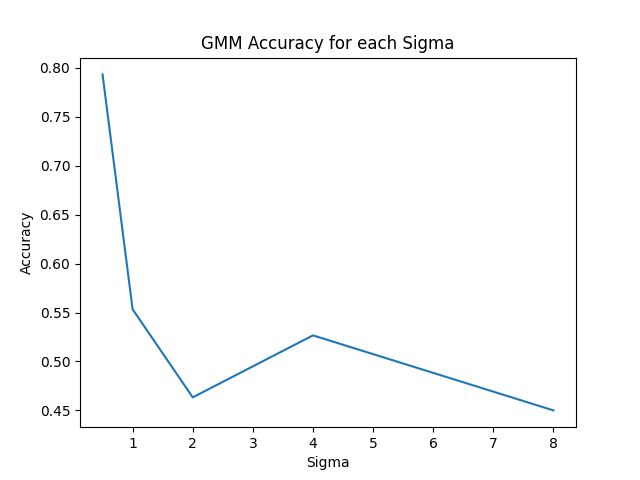
\includegraphics[width=3.15in]{../figs/gmm_accuracy.png} \\
